\documentclass{beamer}
\usepackage{graphicx}
\usepackage{verbatim}
\usepackage{amsmath}
\usepackage{amsfonts}
\usepackage{setspace}
\usepackage{url}
% \usepackage{beamerthemesplit} // Activate for custom appearance

\title{Linear Regression Models\\W4315}
\author{Instructor: Dr. Yang Feng}

\date{Required Text: Applied Linear Regression
Models\\
Authors: Kutner, Nachtsheim, Neter}



\DeclareMathOperator*{\Ave}{\mathbb{E}}
\DeclareMathOperator*{\Var}{Var}

\begin{document}

\frame{\titlepage}


%\frame[t] {
% \frametitle{Not Registered Yet?}
%Fill out the form at\\
%http://tinyurl.com/mqfq95
%\bigskip
%
%Additional books we will draw material from in this course:
%\begin{itemize}
%\item Pattern Recognition and Machine Learning, by Christopher M. Bishop. Springer, 2006.
%\item Bayesian Data Analysis, Second Edition, by Andrew Gelman, John B. Carlin, Hal S. Stern, and Donald B. Rubin, Chapman \& Hall/CRC Texts in Statistical Science
%\end{itemize}
%
%
%
%
%}

\frame[t] {
 \frametitle{Course Description}
Theory and practice of regression analysis, Simple and multiple
regression, including testing, estimation, and confidence
procedures, modeling, regression diagnostics and plots, polynomial
regression, colinearity and confounding, model selection, geometry
of least squares. Extensive use of the computer to analyze data.}

\frame[t] {
 \frametitle{Philosophy and Style}
\begin{itemize}
\item Easy first half.
\item Hard second half.
\item Some digressions from the required book.
\item Understanding == proof (derivation) {\em plus} implementation.
\item Practice makes perfect.
\end{itemize}
}


\frame[t] {
 \frametitle{About me}
\begin{itemize}
\item Operations Research \& Financial Engineering PhD, 2010, Princeton University
\item First time teaching a course...
\end{itemize}
My research
\begin{itemize}
\item High-dimensional Statistical Learning
\item Variable Selection
\item Nonparametric and
Semi-parametric Statistics
\item Bioinformatics
\end{itemize}
}


\frame[t] {
 \frametitle{Course Outline}
 First half of the course is single variable linear regression. 
 \begin{itemize}
 \item Least squares
 \item Maximum likelihood, normal model
 \item Tests / inferences
 \item ANOVA
 \item Diagnostics
 \item Remedial Measures
 \end{itemize}
 
}




\frame[t] {
\frametitle{Course Outline (Continued) }
 Second half of the course is multiple linear regression and other related topics .
\begin{itemize} 
\item Multiple linear Regression
 \begin{itemize}
 \item Linear algebra review
 \item Matrix approach to linear regression
 \item Multiple predictor variables
 \item Diagnostics
 \item Tests
\end{itemize}
\item Other topics (If time permits)
\begin{itemize}
  \item Principle Component Analysis
  \item Generalized Linear Models
  \item Introduction to Bayesian Inference
\end{itemize}
\end{itemize}
}


\frame[t] {
 \frametitle{Requirements}
 \begin{itemize}
 \item Calculus
 \begin{itemize}
 \item Derivatives, gradients, convexity
 \end{itemize}
 \end{itemize}
 \begin{itemize}
 \item Linear algebra
 \begin{itemize}
 \item Matrix notation, inversion, eigenvectors, eigenvalues, rank, quadratic forms
 \end{itemize}
 \end{itemize}
 \begin{itemize}
 \item Probability
 \begin{itemize}
 \item Random variables
 \item Bayes Rule
 \end{itemize}
 \end{itemize}
 \begin{itemize}
 \item Statistics
 \begin{itemize}
 \item Expectation, variance
 \item Estimation
 \item Bias/Variance
 \item Basic probability distributions
 \end{itemize}
 \end{itemize}
 \begin{itemize}
 \item Programming
 \end{itemize}

}


\frame[t] {
 \frametitle{Software}
 \textbf{R} will be used throughout the course and it is required in all homework. An \textbf{R} tutorial session will be given on Sep 22.

Reasons for \textbf{R}:
\begin{itemize}
  \item Completely free software
  \item Available on various systems, PC, MAC, Linux, $\cdots$
\end{itemize}

}

\frame[t] {
 \frametitle{Grading}
 \begin{itemize}
 \item Bi-weekly homework $(25\%)$
 \begin{itemize}
 \item Due every other week
 \begin{itemize}
 \item no late homework accepted
 \end{itemize}
 \item Lowest score will be dropped
 \end{itemize}
  \end{itemize}
 \begin{itemize}
 \item Exams are open book and open notes.
 \item In Class Midterm exam $(30\%)$, Wednesday, Oct 20, 2010 (tentatively).
 \item In Class Final exam $(45\%)$.
 \item Curve
 \end{itemize}

}

\frame[t] {
 \frametitle{Office Hours / Website}
 \begin{itemize}
 \item \url{http://www.stat.columbia.edu/~yangfeng}
 \item Course Materials and homeworks with the due dates will be posted on the course website.
 \item Office hours : Wednesday 2-4pm subject to change
 \item Office Location : Room 1012, SSW Building (1255 Amsterdam Avenue, between 121st and 122nd street)
 \item TA : Qinghua
 \begin{itemize}
 \item TA office hours TBA
 \end{itemize}
 \end{itemize}
}

\frame[t] {
 \frametitle{Why regression?}
 \begin{itemize}
 \item Want to model a functional relationship between an ``predictor variable'' (input, independent variable, etc.)
      and a ``response variable'' (output, dependent variable, etc.)
 \begin{itemize}
 \item Examples?
 \end{itemize}
 \end{itemize}
 \begin{itemize}
 \item But real world is noisy, no $f = ma$
 \begin{itemize}
 \item Observation noise
 \item Process noise
 \end{itemize}
 \item Two distinct goals
 \begin{itemize}
 \item Tests about natural of relationship between predictor variables and response variables
 \item Prediction
 \end{itemize}
 \end{itemize}
}

\frame[t] {
 \frametitle{History}
 \begin{itemize}
 \item Sir Francis Galton, $19^{th}$ century
 \begin{itemize}
 \item Studied the relation between heights of parents and children and noted that the children ``regressed'' to the population mean
 \end{itemize}
 \end{itemize}
 \begin{itemize}
 \item ``Regression'' stuck as the term to describe statistical relations between variables
 \end{itemize}
}

\frame[t] {
 \frametitle{Example Applications}
 Trend lines, eg. Google over 6 mo.
\begin{figure}
  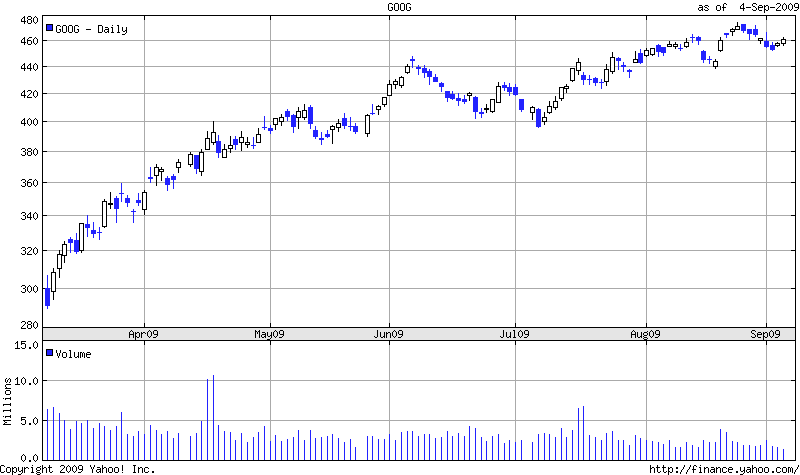
\includegraphics[height=60mm]{google.png}
\end{figure}
}

\frame[t] {
 \frametitle{Others}
 \begin{itemize}
 \item Epidemiology
 \begin{itemize}
 \item Relating lifespan to obesity or smoking habits etc.
 \end{itemize}
 \end{itemize}
 \begin{itemize}
 \item Science and engineering
 \begin{itemize}
 \item Relating physical inputs to physical outputs in complex systems
 \end{itemize}
 \end{itemize}
 \begin{itemize}
 \item Grander

 \begin{center}
 \begin{figure}
  \hspace{-2cm}
  
\includegraphics[height=20mm]{brain.png}
\end{figure}
\end{center}
 \end{itemize}
}

\frame[t] {
 \frametitle{Aims for the course}
\begin{itemize}
\item Given something you would like to predict and some number of covariates
\begin{itemize}
\item What kind of model should you use?
\item Which variables should you include?
\item Which transformations of variables and interaction terms should you use?
\end{itemize}
\item Given a model and some data
\begin{itemize}
\item How do you fit the model to the data?
\item How do you express confidence in the values of the model parameters?
\item How do you regularize the model to avoid over-fitting and other related issues?
\end{itemize}
\end{itemize}

}

\end{document}
